\section{Methodology}

% \subsection{The Urban Heat Island}


\subsection{The SUEWS Model}

The study utilizes an open-source \Gls{lsm} known as the Surface and Urban Energy Balance Scheme (\Gls{suews} from now on, see for example \cite{suews} and \cite{suews2}) through it's bundled Python package \Gls{supy} (\cite{supy2024.7.12}), taking in commonly available meteorological data to model the energy and water balance of the urban surface as shown in Figure~\ref{fig:suews_equations}. Coupled with the heat flux is the modelling of water fluxes that forms the second half of the model's calculation of the energy budget. Thus, the model uses an evaporation-interception approach of the urban surface that feeds into the prior energy balance equation under latent heat flux (Figure~\ref{fig:evapotranspiration_interception_model}, \cite{urban_energy_balance} and \cite{evapotranspiration_interception}). The \Gls{lsm} utilizes multiple sub-models to minimize the amount of forcing data needed to run the model (see \cite{suews} for specifics).

\begin{figure}[bh]
    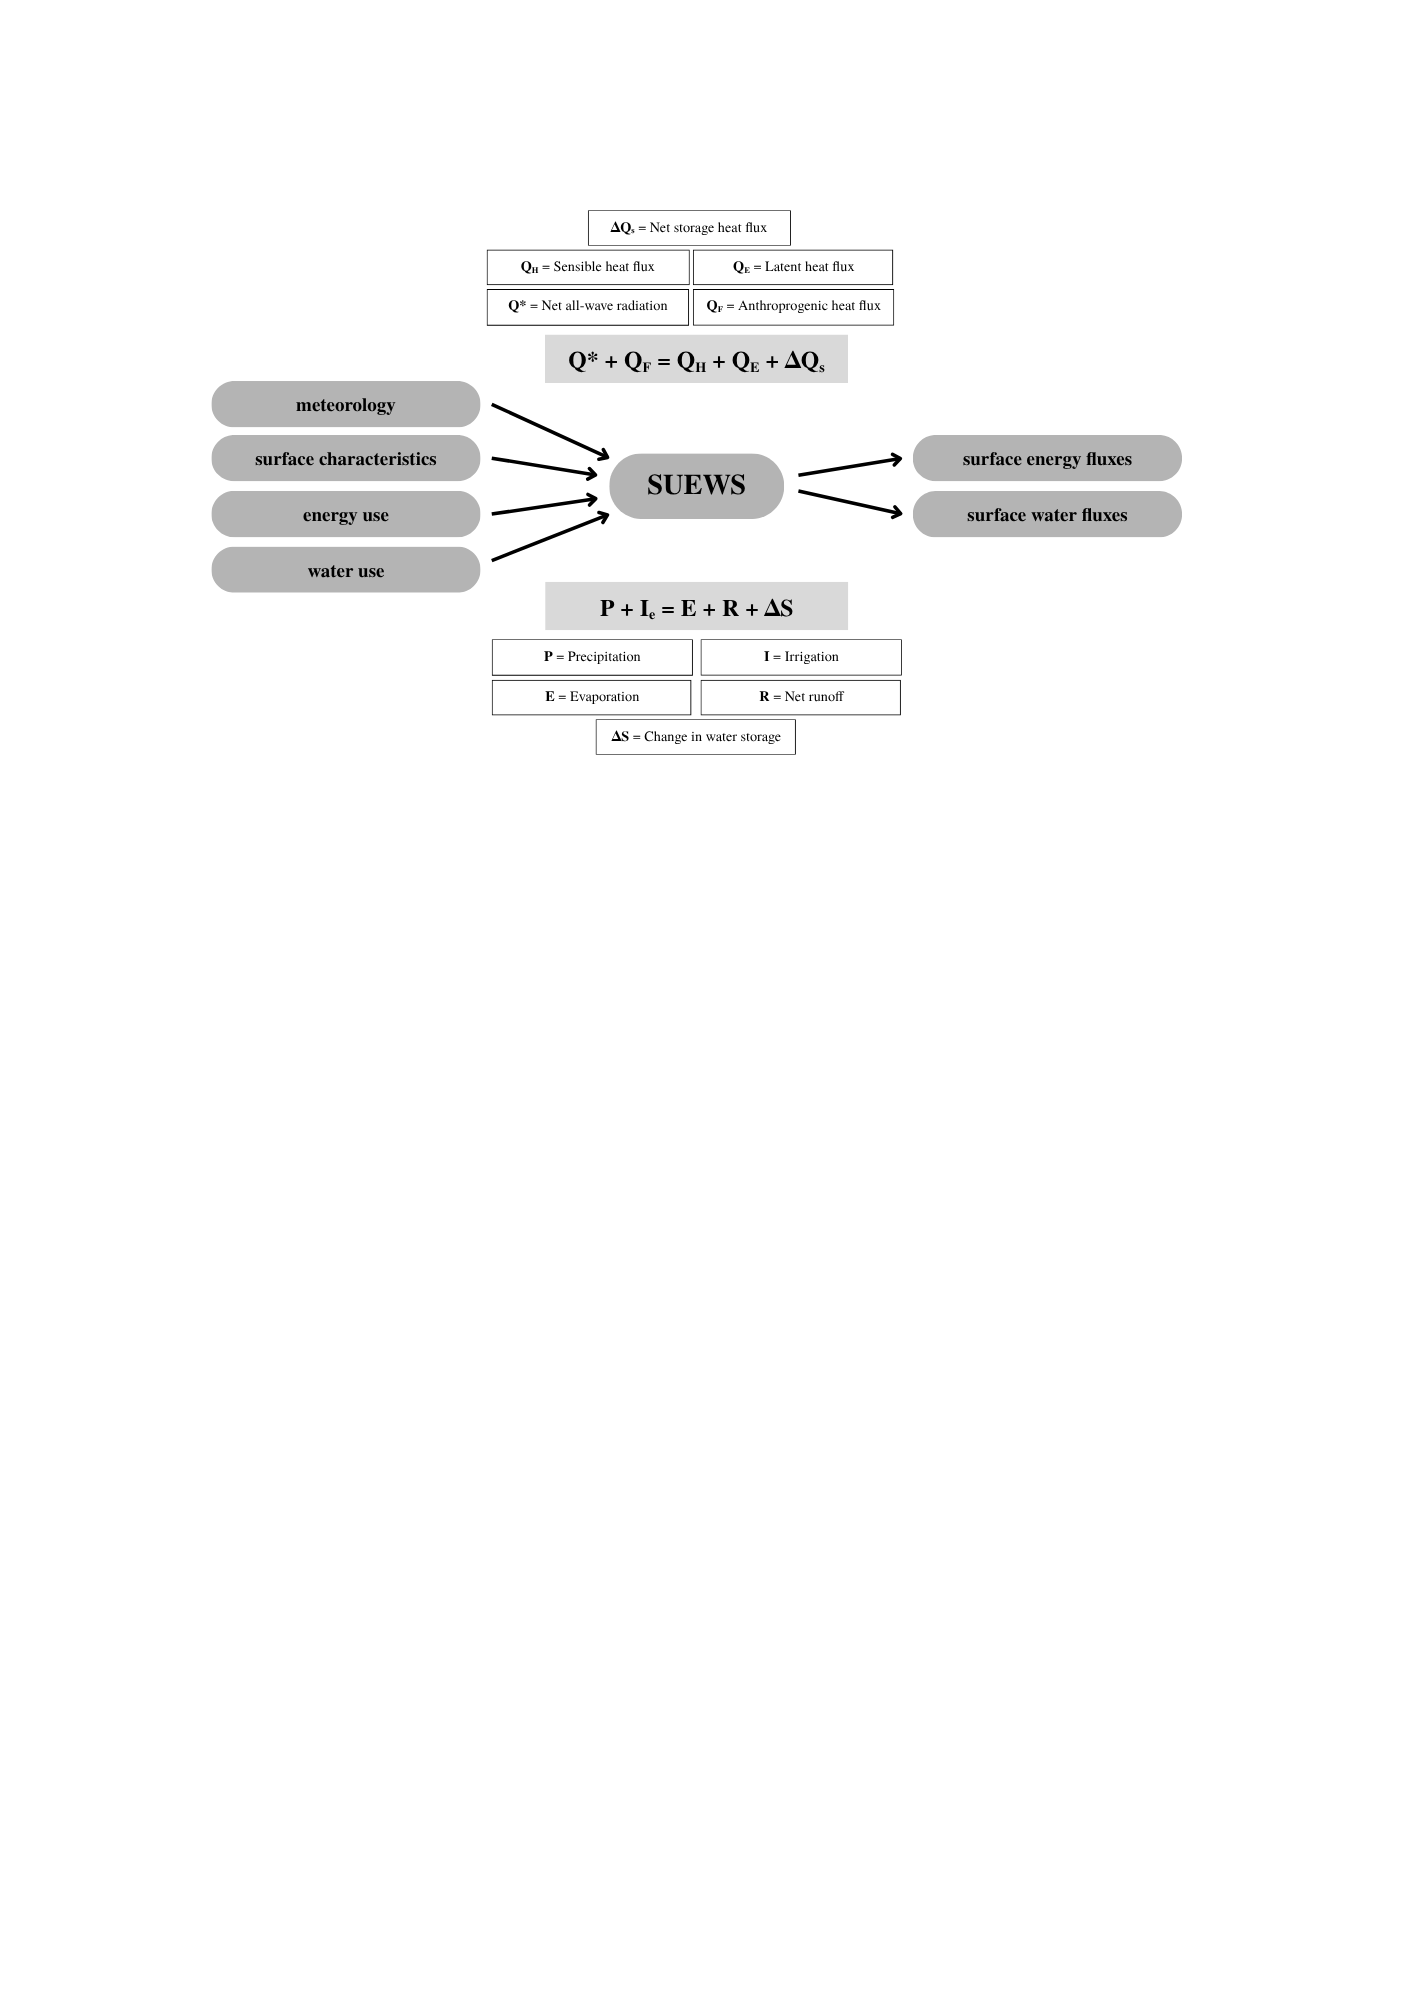
\includegraphics[center, clip, trim = {2cm 17cm 2cm 2cm}]{Image/suews_equations.png}
    \caption{The basic inputs and outputs of SUEWS, adapted from the documentation of \Gls{suews} in \textcite{supy2024.7.12}.}
    \label{fig:suews_equations}
\end{figure}

\begin{figure}[th]
    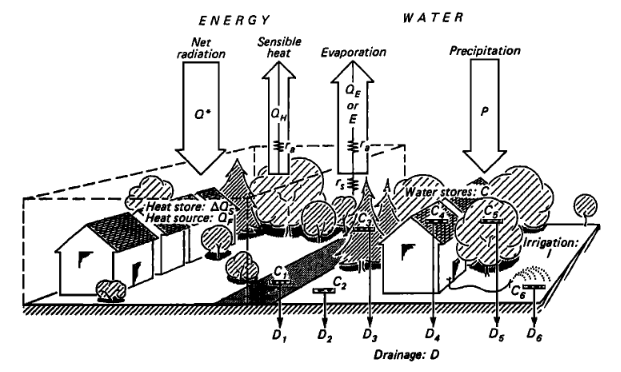
\includegraphics[scale = 0.7, center, clip]{Image/evapotranspiration_interception_model.png}
    \caption{The evapotranspiration model used in SUEWS, taken directly from \textcite[p.1740]{evapotranspiration_interception} where symbols are fully described.}
    \label{fig:evapotranspiration_interception_model}
\end{figure}

Figure~\ref{fig:evapotranspiration_interception_model} showcases the treatment 
single-layer moisture stores 

% 7 different surface cover fractions figure



\subsection{Model Setup}

The \Gls{supy} Global Workflow is a private university GitHub repository by UCL's Department of Disaster and Risk Reduction, where a set of  scripts obtains the necessary input data through the \Gls{gee} API and directly feeds it into \Gls{supy} by simply setting a site's central coordinates. The full process is captured in Figure \ref{fig:process_flowchart}, with the full list of data sources used for the model. \Gls{supy} package version of '2024.7.12.dev' was used for the study (\cite{supy2024.7.12}) with the model running with the default \Gls{supy} sample data for initial soil conditions. The site was run with a spin-up of 2 months to counteract this data unavailability of local soil conditions and to minimize potential errors due to the sensitivity of \Gls{suews} and other \Gls{lsm}s to initial ground and soil conditions (\cite{initial_conditions}). \Gls{supy} was configured to run near the centre of Greater Kuala Lumpur with a total study area of 40km\textsuperscript{2}. Due to computational and data limitations of the \Gls{gee} API, the \Gls{supy} Global LCZ Workflow was ran through multiple instances sequentially to cover the large study area (Figure \ref{fig:process_flowchart}). 2017 forcing in particular was chosen due to a lack of significant weather extremes and to represent a neutral \Gls{enso} state (\cite{mmd_report}). The model takes about 10 hours to complete using the author's personal computer.

% flow chart
\begin{figure}[htb]
    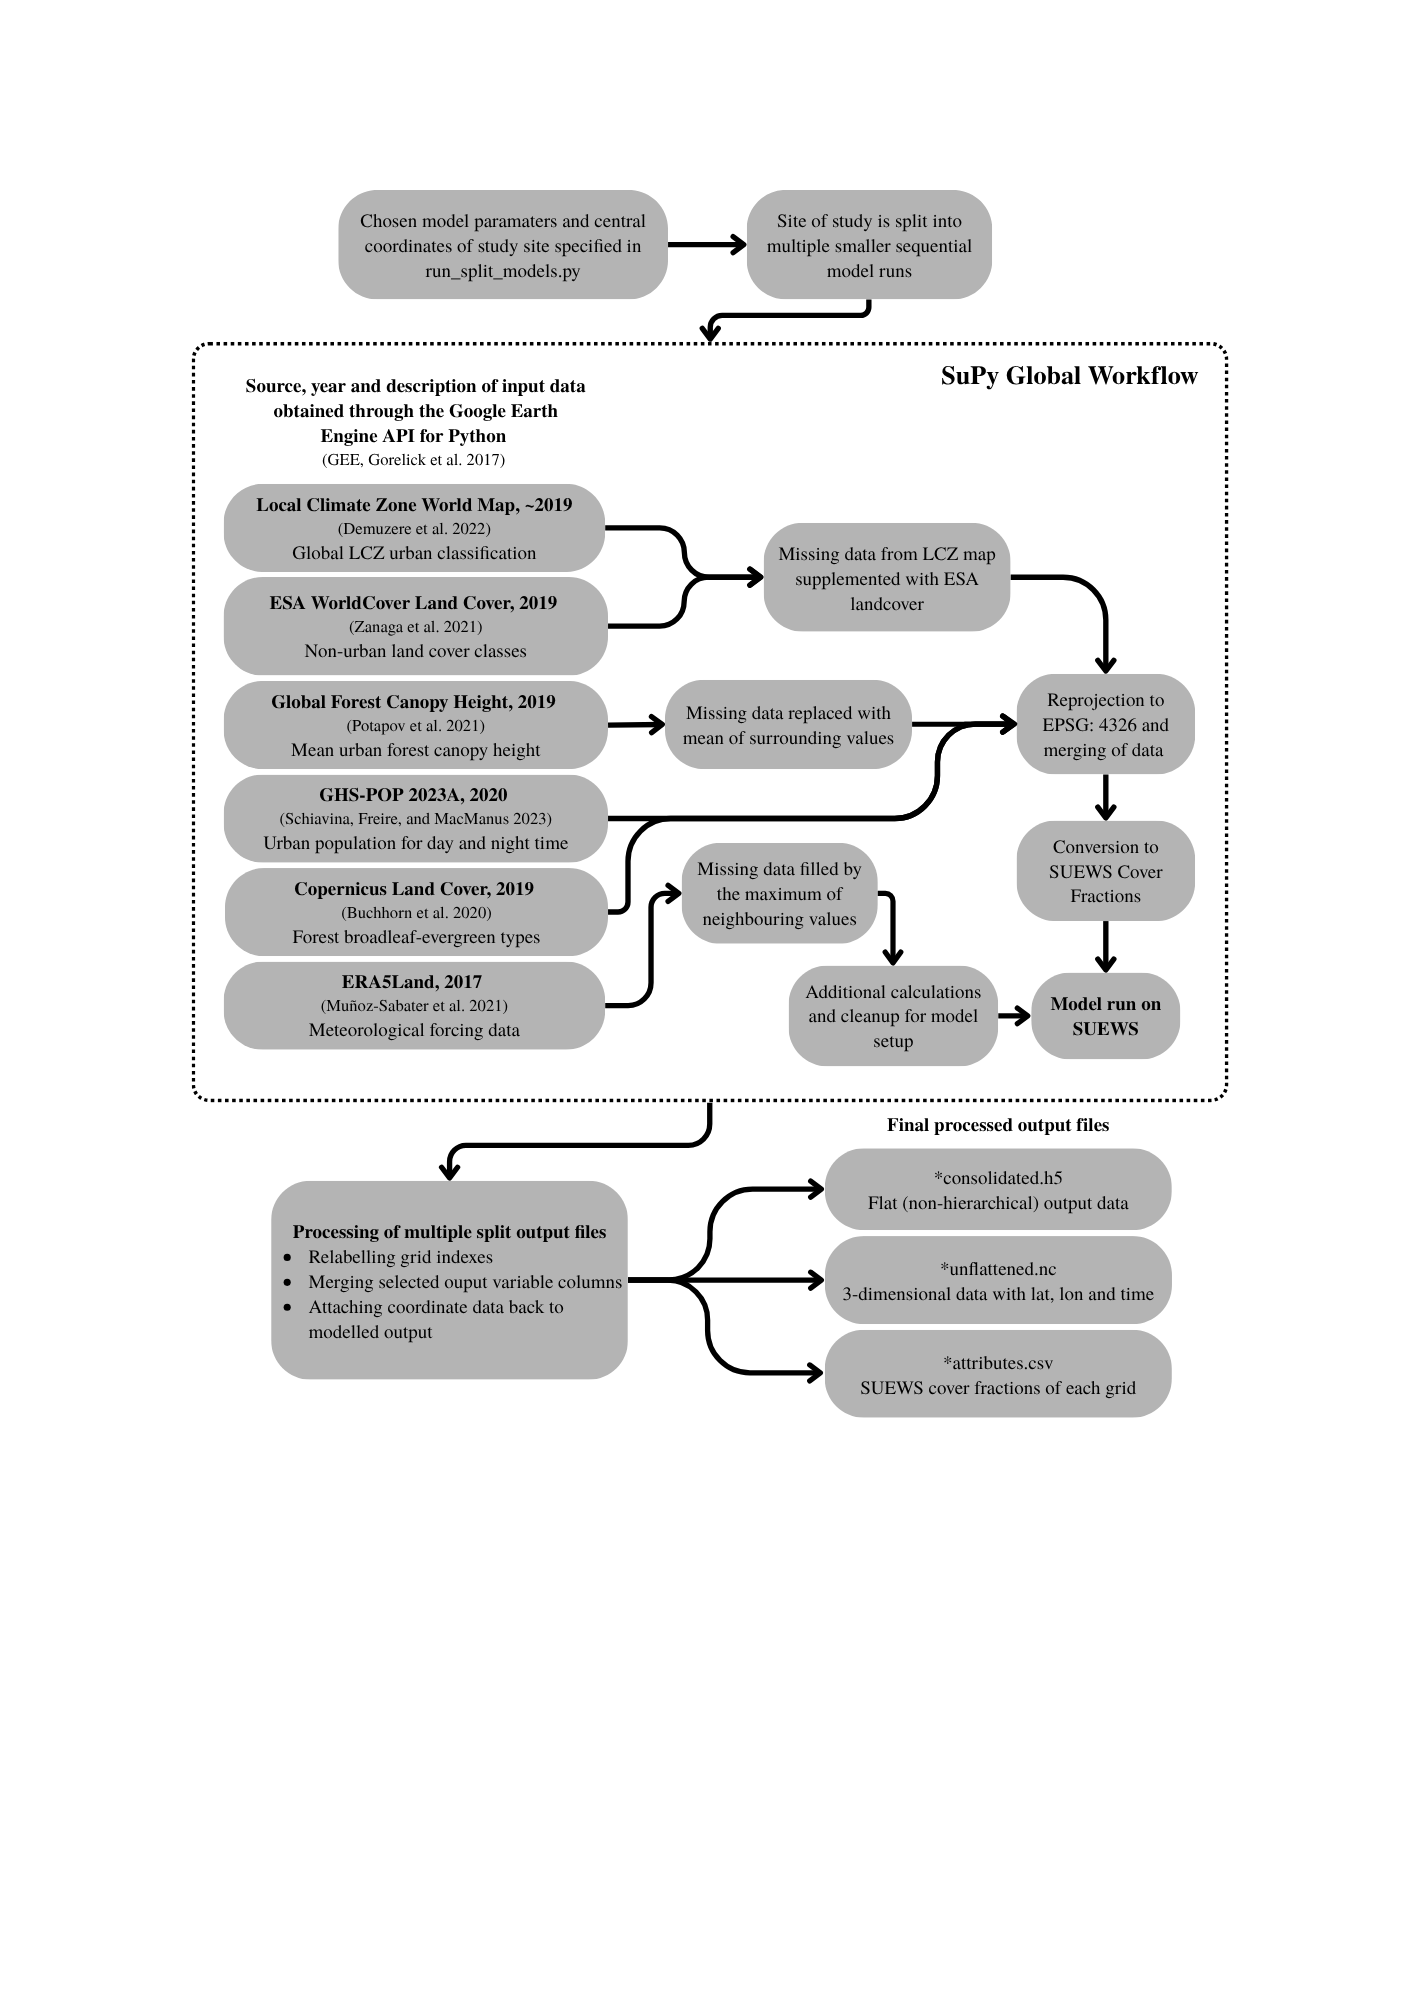
\includegraphics[center, clip, trim = {2cm 5cm 2cm 2cm}]{Image/process_flowchart.png}
    \caption{Flowchart depicting the process of running SUEWS and the \Gls{supy} Global Workflow used for the study, with specific details on data sources and error handling.}
    \label{fig:process_flowchart}
\end{figure}

\subsection{Data Sources}

The workflow relies on a globally available map of \Gls{lcz}, which is an established typology for urban morphology, categorizing urban environments by structure, cover and human activity, resulting in 17 classifications for standardized use in urban heat studies (\cite{lcz}). The Global map of \Gls{lcz}s were derived from a set of human-curated training data that fed into a machine learning classification algorithm of Earth Observation data (\cite{lcz_map}). Land cover information from \textcite{copernicus_lc} was used to identify any missing data which was supplanted through the modal value of surrounding pixels. This \Gls{lcz} map was then fractionated to take into account the model grids being larger than the LCZ map pixels, and then parameterized into author-specified surface cover fractions understandable to \Gls{supy} (Figure \ref{fig:process_flowchart} and see Appendix for tabled parameters). 

Furthermore, \Gls{suews} utilizes population density data from \textcite{popden} to calculate waste heat released through human energy consumption, using a modified approach employed by \textcite{anthropogenic_heat}, where days above and below the baseline temperature of human comfort are termed heating or cooling days. This then provides the model the ability to differentiate the days in terms of energy consumption, thereby providing greater accuracy in estimating energy usage at a finer spatial-temporal scale usually unavailable and difficult to measure directly (\cite{suews}). Figure \ref{} depicts the raw population data and \Gls{lcz}s of the site of study.  The global forest canopy height map by \textcite{forestcanopyheight}) and the ESA WorldCover \textcite{esa_worldcover} are the last two data sources used by the workflow to provide details on the biological components, particularly tree canopy height and the composition of the surface between broadleaf and evergreen forests, which will have a seasonal affect on surface albedo. In the case of \Gls{gkl}, this component is less important as the area is overwhelmingly composed of evergreen forests. 

% LCZ and POPDEN sitemap

\mycomment{
All sourced through the Google Earth Engine API and year of data used and processed through SuPy
    - ERA5Land (2017, author specified), \cite{era5land}
    - GHS-POP 2023A (2020), \cite{popden}
    - LCZ World Map (~2019, multi-year sourced),  \cite{lcz_map}
    - ESA WorldCover 10m v100 Land Cover Fractions (2020), \cite{esa_worldcover} LUC (to identify missing LCZ/Era5Land grtids/pixels and "filling them out"
    - Global Forest Canopy Height (2019), \cite{forestcanopyheight} % Average Height
    - Copernicus Global Land Cover (2019), \cite{copernicus_lc} % for evergreen-broadleaf distinctions
}


\subsection{Suitability}

% previous studies and applicability etc
% add discussion on the role of big data and critically using globally available datasets.
% why SUEWS? alternatives, and current existing papers using the model

The model has been evaluated in the similar tropical urban climate regime of Singapore, using real-world validation data (\cite{demuzere_singapore}). 

\cite{chua_evaluation} 

\subsection{Data Analysis Methods}

% Table of Monsoon dates.

%which noted specific parameterization sensitivities

% add basic UHI equation


% might remove 
% validation and evluation 
        % radiation and heat flux values should look/map reasonable
    
% map making
% The maps were made through a combination of the python package matplotlib and qGIS

% using individual sites as examples

% involving wind speed (10m agl), humidity, and surface temperature variables?

% summary statistics and statistical significance
% statistical significant means

